
\documentclass[12pt,A4paper,titlepage]{article}

%PAQUETES
\usepackage[spanish]{babel}
\usepackage[utf8]{inputenc} %Este paquete permite poner acentos directamente y ees
\usepackage{fontenc}
\usepackage{amsmath}
\usepackage{graphicx}%[pdftex]
\usepackage{graphicx, wrapfig}
\usepackage{fancyhdr}
\usepackage{anysize}
\usepackage{verbatim}
\usepackage{advdate}
\usepackage{colortbl}
\usepackage{amsmath}
\usepackage{amssymb}
\usepackage[dvips,final]{epsfig}
\usepackage{epstopdf}
\marginsize {2.5cm}{2.5cm}{2.5cm}{2.5cm} %Primero margen izquierdo, Segundo margen derecho, Tercero margen superior, Cuarto margen inferior.

%Línea de presentación
\usepackage{fancyhdr}
\pagestyle{fancy}
\fancyhf{}
\fancyhead[L]{Síntesis de Redes Activas - Trabajo Práctico 3}
\fancyfoot[LE,RO]{\thepage}
\fancyfoot[LO]{Armida - Ruiz Tatur}
\renewcommand{\footrulewidth}{0.1pt}

%CARATULA
\begin{document}
\begin{titlepage}

\thispagestyle{empty}


\begin{center}
    
\includegraphics[scale=0.4]{Imagenes Logo/unc_logo.png}
    
\includegraphics[scale=0.4]{Imagenes Logo/fcefyn_logo.jpg}
    \\[1cm]
    \vspace{5pt}
    \LARGE \textbf{Universidad Nacional de Córdoba}\\[0.5cm] 
    \large \textbf{Facultad de Ciencias Exactas, Físicas y Naturales} \\[0.5cm] 
    \large \textbf{Síntesis de Redes Activas}
    \\[0.5cm]
    \large \textbf{Trabajo Práctico Nº3}\\[0.5cm]
    \vspace{60pt}
    \begin{table}[!h]
    \centering
    \begin{tabular}{ll}
    \multicolumn{1}{c}{Nombre} & \multicolumn{1}{c}{DNI} \\
    Armida Abril & 41.436.299  \\
    Ruiz Tatur Manuel & 40.963.553
    \end{tabular}
    \end{table}
    \vspace{20pt}
    \begin{table}[!h]
    \centering
    \begin{tabular}{ll}
    \multicolumn{1}{c}{Docentes} & Ing. Pablo Ferreyra \\
     & Ing. Cesar Reale \\
     
    \end{tabular}
    \end{table}
    \vspace{20pt}
    \large 2023
\end{center}

\end{titlepage}

\newpage
\section{Introducción}
\hspace{1mm} 
En el siguiente informe de laboratorio se trata de explicar las actividades que hemos desarrollado para el diseño de la etapa analógica de una balanza comercial, que puede satisfacer las especificaciones requeridas y que sea capaz de competir comercialmente. Para esto se requiere indicar el circuito propuesto con sus respectivos cálculos analíticos y un estudio económico para minimizar los costos y optimizar el producto, estandarizando los valores y tipos de componentes.

\section{Objetivos}

\hspace{1mm}
Se requiere de una balanza para uso comercial utilizando como sensor una celda de carga. La etapa de amplificación de instrumentación se debe basar en amplificadores operacionales individuales. El trabajo práctico pide también definir las etapas analógicas con su respectivo número de bits necesarios del conversor para que no procese información innecesaria, ya que este valor debe ser compatible con la resolución, el error del sensor y el acondicionamiento de la carga. Para satisfacer estos requerimientos se pueden incluir como datos de salida instrucciones de diseño o procesos que debe realizar el software. Cabe destacar que el principal objetivo del trabajo práctico es realizar una implementación que sea una solución a los problemas planteados pero minimizando los costos de fabricación lo mejor posible ya que se debe diseñar un producto competitivo.

\section{Guía de diseño}
\textbf{Especificaciones técnicas del producto a diseñar:}

    \begin{itemize}
        \item Resolución de 1 gramo.
        \item Temperatura de funcionamiento de $0^{\circ}C$ a $40^{\circ}C$.
        \item Rango máximo de $2Kg$. 	
    \end{itemize}


\newpage
\section{Bloques}
    \subsection{Alimentación}
    \hspace{1mm} Sería impensable colocar una fuente de alimentación directo al puente ya que las fluctuaciones que poseen las mismas introducirán un error demasiado grande, por lo que para ellos se utiliza una fuente de corriente, la cual es mucho más estable. 
    El amplificador operacional conectado con voltaje seguidor obliga a que la tensión de referencia (GND) sea igual a la tensión de carga. Es así que se fuerza a tener \(10~V\) exactos a través de \(R_1 \) entonces, la salida actual será de \(10~V/R_1 \). 

    \bigskip
    \hspace{1mm} El voltaje de salida es extremadamente insensible tanto a la línea como a las variaciones de carga y, puede ajustarse externamente con un efecto mínimo sobre el drift y la estabilidad. El drift es corregido por láser y se obtiene \(2.5~ppm/^\circ C \) tal como lo especifica en el datasheet y con una variación de tensión de \(V_o = 10 \pm 0.0025~V \). Se debe tener en cuenta que la exactitud de la fuente de corriente depende casi exclusivamente de la exactitud absoluta de la resistencia \(R_1 \), siendo la tolerancia y la estabilidad de la resistencia directamente proporcional al drift y a la estabilidad de la temperatura de la fuente de corriente.  Por ejemplo si se utilizara una resistencia de \(50~ppm/ ^\circ C \) (común para resistenias de 1\% de película de metal), la fuente de corriente tendrá un drift de aproximadamente \(50~ppm/ ^\circ C \). Es entonces, que si se sabe cuál es la tensión que se desea tener en el puente y también se conoce la impedancia de entrada del mismo se tiene:
    
    \bigskip
    \begin{equation}
        I_{out} = \frac{10~V}{Z_{cell}~\Omega}=28.57~mA
    \end{equation}
    
    \bigskip
    \hspace{1mm}  Por lo tanto, al necesitar \(10~V\) en la celda de carga, se deberá usar una resistencia del mismo valor de la impedancia de entrada del puente \(Zcell = 350~\Omega \). 

\begin{figure}[!h] 
  \centering
  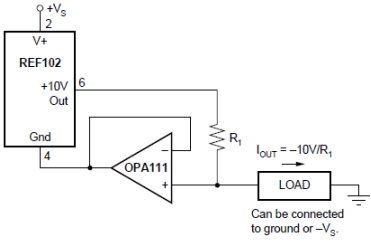
\includegraphics[scale=0.9]{Imagenes/Fuente de corriente.png}
  \caption{\textit{Fuente de corriente.}}
\end{figure}

\newpage

\subsection{Transductor}

\hspace{1mm} Para obtener un determinado nivel de voltaje en función de la masa que se desea medir, se usará como transconductor una \textbf{galga extensiométrica}, también conocida como \textbf{celda de carga}. La galga extensiométrica es básicamente una resistencia eléctrica. El parámetro variable y sujeto a medida es la resistencia de dicha galga. Esta variación de resistencia depende de la deformación que sufre la galga.

\begin{figure}[!h] 
  \centering
  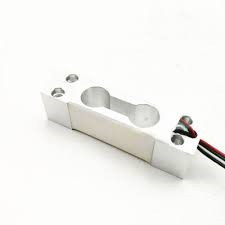
\includegraphics[scale=1]{Imagenes/Celda de carga.jpg}
  \caption{\textit{Celda de carga.}}
\end{figure}

\hspace{1mm} Se parte de la hipótesis inicial de que el sensor experimenta las mismas deformaciones que la superficie sobre la cual está pegada. El sensor está constituido básicamente por una base muy delgada no conductora, sobre la cual está adherido un hilo metálico muy fino, de forma que la mayor parte de su longitud está distribuida paralelamente a una dirección determinada. La resistencia eléctrica del hilo es directamente proporcional a su longitud, o lo que es lo mismo, su resistencia aumenta cuando éste se alarga.

\bigskip
\hspace{1mm} En la galga, medir la tensión requiere la medida exacta de cambios muy pequeños en su resistencia. Para medir tales cambios, las galgas de tensión se utilizan, casi siempre, en una configuración puente con una fuente de excitación de voltaje.

\begin{figure}[!h] 
  \centering
  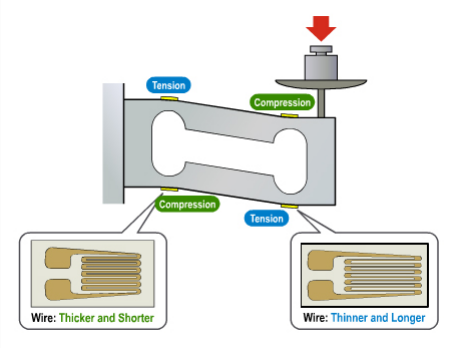
\includegraphics[scale=0.5]{Imagenes/Funcionamiento de la celda de carga.png}
  \caption{\textit{Ilustración del funcionamiento de una celda de carga.}}
\end{figure}

\hspace{1mm} El puente de Wheatstone consiste en cuatro brazos de resistencias con un voltaje de excitación que se aplica a través del puente.

\bigskip
\begin{figure}[!h] 
  \centering
  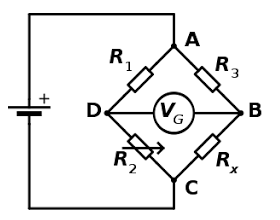
\includegraphics[scale=0.5]{Imagenes/Puente de Wheatstone.png}
  \caption{\textit{Puente de Wheatstone.}}
\end{figure}

\bigskip

\hspace{1mm} Cuando se cumple que
    \begin{equation}
        R_1/R_2 = R_3/R_X
    \end{equation}

la tensión diferencial medida entre los bornes A y B será igual a cero. En esta condición se dice que el puente se encuentra balanceado. Cualquier cambio que se dé en alguna de las resistencias (en este caso, la celda de carga), se traduce en una diferencia de voltaje entre los puntos A y B.
\bigskip

\hspace{1mm} La celda de carga que se utilizó es de la marca FLEXAR SRL, cuyas especificaciones se detallaron a continuación.

\begin{figure}[!h] 
  \centering
  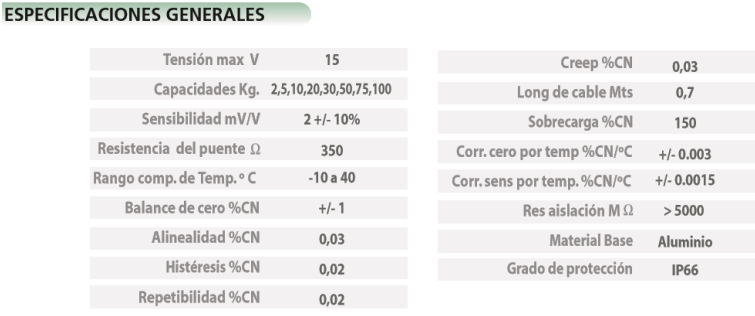
\includegraphics[scale=0.7]{Imagenes/Especificaciones generales.png}
  \caption{\textit{Características de la celda de carga.}}
\end{figure}

 \hspace{1mm} Con dicha sensibilidad de la celda y \(10~V\) netos de alimentación se obtuvo un fondo de escala \(FS = 20\pm 2 ~mV\).
 \hspace{1mm} Si la máxima salida del ADC son \(2~Kg\), cuando haya \(20~mV\) de tensión diferencial entonces se obtienen \(2~Kg\) a la salida. Esto quiere decir que se consiguen 2000 escalones de cuantización, donde cada escalón equivale a \(1~g\), es decir, \(10~uV\) de tensión diferencial. Para esto, se necesita un conversor A/D de mínimo 11 bits. Pero se optó en elegir uno de 12 bits para tener la posibilidad de cuantificar mejor algunos errores que pueden ser corregidos por software. 

\subsection{Amplificación}
\hspace{1mm} La celda de carga entrega una señal diferencial a su salida que deberá ser amplificada. Esta señal luego será transformada por un conversor analógico/digital y mostrada a través de un display que proporciona la información necesaria para los usuarios. 

\bigskip
\hspace{1mm} La etapa de amplificación será desarrollada mediante un arreglo de operacionales discretos que en conjunto deben funcionar como un amplificador de instrumentación. La elección del mismo depende de sus dos etapas, una primera que posee dos amplificadores operacionales en simetría cuya función es bufferear ambas entradas y no agregar errores apreciables debido a la configuración de los mismos (se cancelan entre ambos).  Los errores que pueden aparecer sólo se deben a la construcción física de los amplificadores operaciones, por lo que se seleccionarán operacionales apareados a razón de disminuir al máximo este inconveniente.

\begin{figure}[!h] 
  \centering
  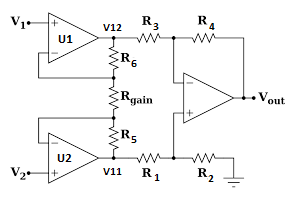
\includegraphics[scale=1.3]{Imagenes/Amplificador de instrumentación.png}
  \caption{\textit{Amplificador de instrumentación.}}
\end{figure}

\hspace{1mm} Más adelante se demostrará la necesidad de que \(R_1 \cdot R_4 = R_2 \cdot R_3\), para tener simetría en la etapa de amplificación \(R_5 = R_6\).

\bigskip
\hspace{1mm} Se comenzó analizando el circuito genérico sin simplificaciones. Entonces, aplicando el principio de superposición, la salida \(V_{out}\) será.

\bigskip
\begin{equation}
\label{superp}
V_{out} = \frac{V_{out}}{V_{11}} |_{V_{12} = 0} + \frac{V_{out}}{V_{12}}|_{V_{11}=0}
\end{equation}

\bigskip
\hspace{1mm} De la cual, la ganancia con respecto a cada entrada resultó.

\begin{equation}
  V_{out}|_{V_{11}=0} = -V_{12} \cdot \frac{R_4}{R_3} \quad y \quad   V_{out}|_{V_{12}=0} = V_{11} \cdot \frac{R_2}{R_1 + R_2} 
\cdot \left(1+\frac{R_4}{R_3}\right)
\end{equation}

\bigskip

\hspace{1mm} Reemplazando en la ecuación principal \(V_{out}\) se tiene.

\bigskip

\begin{equation}
    V_{out} = V_{11} \frac{R_2}{R_1 + R_2} \cdot \left(1 + \frac{R_4}{R_3}\right) - V_{12} \frac{R_4}{R_3}
\end{equation}

\bigskip
\hspace{1mm} Para el caso donde \(V_2 = 0\), las ecuaciones quedan de la siguiente forma.
\bigskip
\begin{equation}
    V_{11} = V_1 \left(1 + \frac{R_5}{R_{gain}}\right)
\end{equation}

y

\begin{equation}
    V_{12} = -V_{11} \cdot \frac{R_{gain}}{R_5 + R_{gain}}
\end{equation}

\bigskip
\hspace{1mm} Si se realiza sustitución se obtiene.

\begin{equation}
    V_{12} = -V_1 \frac{R_{gain}}{R_5 + R_{gain}} \left(1 + \frac{R_5}{R_{gain}}\right)
\end{equation}

\bigskip
\hspace{1mm} Siendo así la salida cuando \(V_2 = 0\) igual a:

\bigskip
\begin{equation}
    V_{out}|_{V_2=0} = V_1 \cdot \left(1 + \frac{R_5}{R_{gain}}\right) \cdot \frac{R_2}{R_1 + R_2} \cdot \left(1 + \frac{R_4}{R_3}\right) + V_1 \frac{R_5}{R_{gain}} \cdot \frac{R_4}{R_3}
\end{equation}

\bigskip
\hspace{1mm} Luego, se realiza un análisis análogo para el caso donde \(V_1 = 0\). Se tiene:

\begin{equation}
    V_{12} = V_2 \left(1 + \frac{R_6}{R_{gain}}\right)
\end{equation}

\hspace{1mm} y

\begin{equation}
    V_{11} = -V_{12} \frac{R_5}{R_6 + R_{gain}}
\end{equation}

\bigskip
\hspace{1mm} Si se sustituye queda.

\begin{equation}
    V_{11} = -V_2 \frac{R_5}{R_6 + R_{gain}} \left(1 + \frac{R_6}{R_{gain}}\right)
\end{equation}

\bigskip
\hspace{1mm} Siendo así la salida cuando \(V_1 = 0\)

\bigskip
\begin{equation}
    V_{out}|_{V_1=0} = V_2 \cdot \frac{R_5}{R_{gain}} \frac{R_2}{R_1 + R_2} \cdot \left(1 + \frac{R_4}{R_3}\right)  - V_2 \cdot \left(1+\frac{R_6}{R_{gain}}\right) \cdot \frac{R_4}{R_3}
\end{equation}

\bigskip
\hspace{1mm} Por lo que la salida total está dada por la suma de las ecuaciones (9) y (13).

\bigskip
\hspace{1mm} Se tomó el caso ideal, donde se cumple que \(R_1 \cdot R_4 = R_2 \cdot R_3\) y que \(R_5 = R_6\) por lo tanto las expresiones (9) y (13) quedan simplificadas de la siguiente manera.

\begin{equation}
    V_{out}|_{V_2=0} = V_1 \cdot \left(1 + \frac{R_5}{R_{gain}}\right) \cdot \frac{R_2}{R_1} + V_1 \cdot \frac{R_5}{R_{gain}} \cdot \frac{R_2}{R_1}
\end{equation}

\bigskip
\begin{equation}
    V_{out}|_{V_2=0} = V_1 \cdot \frac{R_2}{R_1} \cdot \left(1 + 2 \frac{R_5}{R_{gain}}\right)
\end{equation}

\bigskip
\begin{equation}
    V_{out}|_{V_1=0} = V_2 \cdot \left(1 + \frac{R_5}{R_{gain}}\right) \frac{R_2}{R_1} + V_2 \cdot \frac{R_5}{R_{gain}} \cdot \frac{R_2}{R_1}
\end{equation}

\bigskip
\begin{equation}
    V_{out}|_{V_1=0} = V_2 \cdot \frac{R_2}{R_1} \cdot \left(1 + 2 \frac{R_5}{R_{gain}}\right)
\end{equation}

\bigskip
\hspace{1mm} Si se realiza la suma de las dos ecuaciones se tiene la salida total. A continuación se tiene lo especificado:

\begin{equation}
    V_{out}=\left[V_1-V_2\right] \cdot \frac{R_2}{R_1} \cdot \left(1+2\frac{R_5}{R_{gain}}\right)
\end{equation}

\bigskip
y la ganancia del amplificador entonces será,

\begin{equation}
    A_v=\frac{V_{out}}{V_1-V_2}=\frac{R_2}{R_1} \cdot \left(1+2\frac{R_5}{R_{gain}}\right)
\end{equation}

\bigskip
\hspace{1mm} Si se utiliza un conversor con un fondo de escala de \(3~V\) y se lo divide por la máxima salida que se puede obtener (\(20~mV\)), se tendrá la ganancia total del circuito de amplificación que debe ser aproximadamente 150 veces. Como se mencionó anteriormente, para no amplificar el ruido y los errores de los amplificadores de la primer etapa, se utilizará el segundo amplificador como buffer. Para esto mismo se necesita que:

\begin{equation}
    R_1=R_2=1~K\Omega
\end{equation}

\bigskip
\hspace{1mm} Por lo que la expresión de la ganancia se reduce a,

\begin{equation}
    A_v=1+2\frac{R_5}{R_{gain}}=150
\end{equation}

\hspace{1mm} Por lo tanto, con la relación anterior, si \(R_5=16.4~K\Omega \) entonces, \(R_{gain}=200~\Omega \).

\bigskip
\hspace{1mm} Con el valor de estas resistencias no se tiene una ganancia exacta de 150 veces, sino que se tiene un pequeño error debido al redondeo del valor de las mismas. Este error, en conjunto con el error que introducen las tolerancias de las resistencias, el cual se analizará más adelante, puede ser solucionado utilizando un trimmer como \( R_{gain} \) para así poder obtener exáctamente la ganancia de 150 veces.

\bigskip
\hspace{1mm} Por último, los amplificadores a utilizar serán los integrados en el LMC6064, cuyas caracterísitcas son:

\begin{itemize}
    \item \(RRMC=85~dB\)
    \item \(V_{os} = 100~uV \)
    \item \(I_{pol} = 0.01~pA \)
    \item \(I_{os}=0.005~pA \)
    \item \(A_d(0)=140~dB \)
\end{itemize}



\section{Análisis de Errores}

\subsection{Errores de la Fuente de Corriente}

\hspace{1mm} En primera instancia, el datasheet del componente REF102 expecifica que la tensión de salida es.
\bigskip
\begin{equation}
    V_{out} = 10 \pm 0.0025~V
\end{equation}

\bigskip
\hspace{1mm} La temperatura juega un rol importante en la variación de la corriente que circula por la carga. Si \(V_o\) es la tensión a bornes de la celda, se tiene que si se usan resistencias con tolerancia del \(0.1\% (10~ppm / ^\circ C)\) se encuentra que,

\bigskip
\begin{equation}
    V_o = I_{out} \cdot Z_{cell}
\end{equation}

\bigskip
\hspace{1mm} Con la tolerancia especificada y siendo \(Z_{cell}=350\)
\bigskip
\begin{equation}
    350~\Omega \pm 0.1\% (+10~ppm /ºC)
\end{equation}

\bigskip
\hspace{1mm} Dando como resultado para 0\(^\circ \)C y 40\(^\circ\) lo siguiente.
 
\bigskip
\begin{equation}
    349.615~\Omega < R_1 < 350.285~\Omega \hspace{2mm} a \hspace{2mm} 0^\circ C
\end{equation}

\begin{equation}
    349.636~\Omega < R_1 < 350.364~\Omega\hspace{2mm} a\hspace{2mm} 40^\circ C
\end{equation}

\bigskip
\hspace{1mm} Se tomó la mayor variación siendo así.

\bigskip
\begin{equation}
    I_{out}=\frac{350.364~\Omega-349.615~\Omega} \cdot {350~\Omega} \cdot 100=0.21\%
\end{equation}

\bigskip
\hspace{1mm} Por lo que la corriente \(I_{out}\) será función de esta variación y tendremos que.

\begin{equation}
    28.51~mA < I_{out} < 28.63~mA
\end{equation}

\bigskip
\hspace{1mm} Entonces el valor de variación de la tensión de salida es.

\bigskip
\begin{equation}
    \Delta V_{out} = (I_{out} \pm 0.21\%) \cdot 350~\Omega = 0.042~V
\end{equation}

\bigskip
\hspace{1mm} Siendo \(42~mV\) la variación máxima entre el intervalo generado por \( (9.9785 ; 10.0205)~V \) que es producido por la variación de las resistencias.

\bigskip
\begin{equation}
    \Delta V_{out} = \pm 21~mV
\end{equation}

\bigskip
\hspace{1mm} Ahora si se le incluye la variación de tensión brindada por el datasheet \((\pm 2.5~mV)\) la variación de tensión es.

\bigskip
\begin{equation}
    \Delta V_{out} = \pm 23.5~mV
\end{equation}

\bigskip
\hspace{1mm} Donde se nota la variación de la resistencia con respecto a la temperatura y por ende la variación de la tensión es pequeña, quedando así fuera del análisis, por lo que se tomó como ideal.

\subsection{Errores en la celda de carga}

\hspace{1mm} La celda de carga junto con el puente de Wheatstone poseen una serie de errores, los cuales algunos de ellos pueden ser corregidos o minimizados por software y otros, limitarán la precisión del circuito de salida. Entonces, 

\begin{itemize}
    \item \textbf{Variación de la sensibilidad:} este parámetro indica la desviación de la sensibilidad. Para minimizarlo, se toma la lectura de la celda con una carga patrón y así se conoce cuál es la sensibilidad exacta de la misma. 
    
    \begin{equation}
        \Delta S =\pm 0.2~mV/V
    \end{equation}

    Cómo la alimentación del circuito es de \(10~V\) se tiene que:
    
    \begin{equation}
        \Delta S|_{max}=\pm 2~mV\equiv \pm 200~g
    \end{equation}
    
    \bigskip
    \item \textbf{Zero Balance:} cuando no hay carga sobre la balanza, la diferencia entre las resistencias nominales del puente producirán un voltaje diferencial. Esto también puede ser corregido por software si se consigue la lectura del valor de la balanza en vacío. 
    
    \begin{equation}
        \Delta Z=\pm 1 \%FS = \pm 0.2~mV \equiv \pm 20~g
    \end{equation}
    
    \bigskip
    \item \textbf{No linealidad de la salida:} A medida que la carga varía entre los \(0~kg\) y los \(2~kg\), la salida diferencial no es perfectamente lineal. Para minimizar este error, se toma una serie de medidas con cargas patrones que determinarán la curva real de salida. Luego se podrá corregir por software.
    
    \begin{equation}
        \Delta NL = \pm 0.03 \%FS = \pm 4~\mu V \equiv \pm 0.4~g
    \end{equation}

    \bigskip
    \item \textbf{Histéresis de la salida:} Este error presenta una desviación en la lectura según la dinámica de las mediciones, en donde se haya una diferencia entre medir una carga liviana y después otra más pesada, con medir una pesada y luego una más liviana. 
    
    \begin{equation}
        \Delta H =\pm 0.02 \% FS = \pm 6~\mu V \equiv \pm 0.6~g
    \end{equation}

    \bigskip
    \item \textbf{Desplazamiento del cero con la temperatura:} Este parámetro indica cuánto es el corrimiento del valor en vacío en función de la temperatura. Una forma de disminuir este error es medir la temperatura constantemente y corregirla por software.
    
    \begin{equation}
        \Delta ZT= \pm 0.003 \% \frac{FS}{1 ^\circ C}
    \end{equation}
    
    \bigskip
    En el peor de los casos, es decir, si la balanza se encuentra a unos \(40 ^\circ C \), se tiene que:
    
    \begin{equation}
        \Delta ZT|_{max} = \pm 24~\mu V \equiv \pm 2.4~g
    \end{equation}
    
    \bigskip
    \item \textbf{Creep:} Este error indica la variación a al salida de la celda cuando está sometida a un esfuerzo físico con un peso constante por un largo período de tiempo. Para evitar este error se podría tomar por software el tiempo en el que la balanza es sometida a un mismo peso y resetear la misma, o apagarla, si sobrepasa un determinado tiempo.
    En este caso, el fabricante especifica este valor como un porcentaje del fondo de escala para \(30~min\),
    
    \begin{equation}
        \Delta C = \pm 0.03 \% FS = \pm 6~\mu V \equiv \pm 0.6~g
    \end{equation}
    
    \bigskip
    Todos estos parámetros se encuentran especificados en las características de la celda de carga elegida anteriormente. 
\end{itemize}

\subsection{\textbf{Error en etapa de amplificación}}
\subsubsection{\textbf{Error por tensión de offset}}
\hspace{1mm} Se tiene la siguiente ecuación,

\begin{equation}
    \Delta V_o |_{V_{os}} = \Delta V_o |_{V_{os1}} + \Delta V_o |_{V_{os2}} + \Delta V_o |_{V_{os3}}
\end{equation}

\bigskip
\hspace{1mm} Donde \(V_{os1}\) es la tensión de offset del amplificador con entrada \(V_1\), \(V_{os2}\) es la tensión de offset del amplificador con la entrada \(V_2\), y \(V_3\) es la tensión de offset del amplificador diferencial. A continuación se detalla cada una por separado,

\begin{equation}
    \Delta V_o|_{V_{os1}} = \frac{R_2}{R_1} \cdot \left(\frac{R_5}{R_{gain}} + 1\right) \cdot V_{os1}
\end{equation}

\bigskip
\begin{equation}
    \Delta V_o|_{V_{os2}} = \frac{R_2}{R_1} \cdot \left(\frac{R_5}{R_{gain}} + 1\right) \cdot V_{os2}
\end{equation}

\bigskip
\begin{equation}
    \Delta V_o|_{V_{os3}} = \left(\frac{R_2}{R_1} + 1\right) \cdot V_{os3}
\end{equation}

\bigskip
\hspace{1mm} Realizando los cálculos se obtiene un error total de tensión de offset de,
\begin{equation}
    \Delta V_o|_{V_{os}} = \pm 15.3~mV
\end{equation}

\subsubsection{\textbf{Error por corriente de polarización}}
\hspace{1mm} Las corrientes de offset se presentan en los tres amplificadores. Se comenzó analizando la salida existente debido a las corrientes de polarización de los primeros dos amplificadores, tomando el tercer amplificador como ideal.

\bigskip
\hspace{1mm} Para este caso se tiene,

\begin{equation}
    V_1^+ = V_2^+ = I_p^+ \frac{Z_{cell}}{2}
\end{equation}

\begin{equation}
    V_1^- = V_2^- = I_p^- \cdot \left[R_5//(R_5 + R_{gain})\right]
\end{equation}

\bigskip
\hspace{1mm} Por simetría y asumiendo que \(R_6 = R_5\), la salida del amplificador es,

\begin{equation}
    V_{11} = V_{12} = (V^+ - V^-) \cdot \left(1 + \frac{R_5}{R_{gain}}\right)
\end{equation}

\bigskip
\hspace{1mm} Por lo que la salida del amplificador de instrumentación resulta,

\begin{equation}
    V_{out}|_{AO1.AO2} = 2(V^+ - V^-) \cdot \left(1+\frac{R_5}{R_{gain}}\right) \cdot \frac{R_2}{R_1} = 12~nV
\end{equation}

\bigskip
\hspace{1mm} La salida del amplificador de instrumentación debido a las corrientes de polarización del tercer amplificador esta dada por,

\begin{equation}
    V_{out}|_{AO3} = I_p^+ (R_1 // R_2) - I_p^- (R_3 // R_4)
\end{equation}

\bigskip
\hspace{1mm} Donde se pone en evidencia la necesidad de que \(R_1 = R_3\) y \(R_2 = R_4\), entonces,
\begin{equation}
    V_{out}|_{AO3} = I_{os} \cdot (R_1 // R_2) = 2.5~pV
\end{equation}

\bigskip
\hspace{1mm} Siendo este valor casi imperceptible por el sistema, por lo que se puede suponer que el error producido por las corrientes de polarización es casi nulo.

\subsubsection{\textbf{Error por RRMC finita}}

\hspace{1mm} Para calcular el valor de este error se utiliza la siguiente fórmula.

\begin{equation}
    \Delta V_o|_{RRMC} = \Delta V_o|_{RRMC1} +\Delta V_o|_{RRMC2} +\Delta V_o|_{RRMC3}
\end{equation}

\bigskip
\hspace{1mm} El desarrollo de cada unos de sus términos resulta,

\begin{equation}
    \Delta V_o|_{RRMC1} = - \frac{FS}{RRMC1}
\end{equation}

\begin{equation}
    \Delta V_o|_{RRMC2} = - \frac{FS}{RRMC2}
\end{equation}

\begin{equation}
    \Delta V_o|_{RRMC3} = - \frac{FS}{\left(1 + 2 \frac{R_5}{R_{gain}}\right) \cdot RRMC3}
\end{equation}

\bigskip
\hspace{1mm} Los primeros amplificadores serán integrados duales, lo que hace que el error producido por RRMC finita se anule entre ambos, por lo que el error producido por RRMC finita resulta ser igual a,

\begin{equation}
    \Delta V_o|_{RRMC} = 1.12~\mu V
\end{equation}

\subsubsection{\textbf{Error total de la etapa amplificadora}}
\hspace{1mm} Se considera que las resistencias son ideales, es decir con una tolerancia de 0\%, siendo así que el error total de esta etapa amplificadora es afectado casi en su totalidad por las tensiones de offset en los amplificadores. Por lo que,
\begin{equation}
    \Delta V_o = \pm 15.3~mV
\end{equation}

\subsection{Error por tolerancia de las resistencias}
\hspace{1mm} En los análisis previos se consideró que las resistencias eran ideales y que no presentaban ninguna variación en su valor. En la práctico esto no es cierto, las mismas difieren de su valor ideal en un rango especificado por la tolerancia. 

A continuación se tomará el peor de los casos, en donde las resistencias difieren de su valor ideal en el máximo valor posible. Se define \(\alpha \) al valor del coeficiente de tolerancia,

\begin{equation}
    \alpha = \frac{tolerancia[\%]}{100}
\end{equation}


\bigskip
Esta disparidad en los valores de las resistencias generarán dos problemas, por un lado una variación de ganancia y por el otro, una disminución de la relación de rechazo de modo común.

\newpage
\subsubsection{Variación de la ganancia}
\hspace{1mm} En el peor de los casos se tendrá que los valores de las resistencias del amplificador de instrumentación serán los siguientes, 

\begin{equation}
  \label{eq4}
\begin{cases}  R_2^{'} = R_2(1 - \alpha)
		\\R_1^{'} = R_1(1+\alpha)
		\\R_4 =  R_2(1+\alpha)
		\\R_3 =  R_1(1-\alpha)
		\\R_5^{'} =  R_5(1+\alpha)
		\\R_6 =  R_5(1-\alpha)
\end{cases}
\end{equation}

\bigskip
\hspace{1mm} La tolerancia de la resistencia \(R_{gain}\) no se consideró dentro de los cálculos ya que la variación del resultado es insignificante.

\hspace{1mm} Para dichos valores de resistencia se tiene,

\begin{multline}
    V_{out}|_{V_2=0} =  V_1 \cdot \left(1 + \frac{R_5 (1+\alpha)}{R_{gain}}\right) \cdot \frac{R_2 (1-\alpha)}{R_2 (1-\alpha) + R_1 (1 + \alpha)} \cdot \left(1 + \frac{R_2 (1 + \alpha)}{R_1 (1 - \alpha)}\right) 
    \\
    \\ + V_1 \cdot \frac{R_5 (1 - \alpha)}{R_{gain}} \frac{R_2 (1 + \alpha)}{R_1 (1 - \alpha)}    
\end{multline}

\begin{multline}
    V_{out}|_{V_1=0} =  V_2 \cdot \left(1 + \frac{R_5 (1+\alpha)}{R_{gain}}\right) \cdot \frac{R_2 (1-\alpha)}{R_2 (1-\alpha) + R_1 (1 + \alpha)} \cdot \left(1 + \frac{R_2 (1 + \alpha)}{R_1 (1 - \alpha)}\right) 
    \\
    \\ + V_2 \cdot \frac{R_5 (1 - \alpha)}{R_{gain}} \frac{R_2 (1 + \alpha)}{R_1 (1 - \alpha)}    
\end{multline}

\bigskip
\hspace{1mm} Se toma que \(R_1 = R_2\), aunque entre ellos habrá una diferencia de valores del valor de,
\begin{equation}
    \frac{R_2}{R_1} = \frac{(1 + \alpha)}{(1 - \alpha)}
\end{equation}

\bigskip
\hspace{1mm} Sumando las salidas y desarrollando, se obtiene,

\begin{multline}
    V_{out} = \frac{(V_1 - V_2)}{(1 - \alpha)^2} \cdot \left(\frac{R_5 (1 + \alpha)}{R_{gain}} \cdot (1 + \alpha^2) + \frac{R_5 (1 - \alpha)}{R_{gain}} \cdot (1 + \alpha)^2)\right)
    \\
    \\ + \frac{1}{(1 - \alpha)^2} \cdot (V_1 (1 +\alpha^2) - V_2 (1 + \alpha)^2)
\end{multline}

\bigskip
\hspace{1mm} Luego, se cuantifica la salida con diferentes valores de tolerancia, siendo,
\begin{equation}
    (V_1 - V_2)|_{max} = 20 ~mV
\end{equation}

\bigskip
Entonces el máximo error producido por una tolerancia del 1\% es.

\begin{equation}
    \Delta V_{out} = \pm 50.9 ~mV
\end{equation}

\bigskip
\hspace{1mm} Mientras que con una tolerancia del 0.1\%, el error es.

\begin{equation}
    \Delta V_{out} = \pm 11.09 ~mV
\end{equation}

\subsubsection{Disminución del RRMC}
\hspace{1mm} La tolerancia de las resistencias producirá una disminución en la relación de rechazo en modo común del amplificador de instrumentación en su conjunto. La RRMC está afectada por la siguiente relación,

\begin{equation}
    \frac{1}{RMMC_{tot}}=\frac{-1}{RRMC_1}+\frac{1}{RRMC_2}+\frac{1}{1+2\frac{R_5}{R_{gain}}}\left(\frac{1}{RRMC_3}+\frac{1}{RRMC_R}\right)
\end{equation}

\bigskip
Como se mencionó anteriormente, si se utilizan dos amplificadores duales integrados para la primera etapa, en donde ambos tengan la misma RRMC, los dos primeros términos de la Ec.(60) se anulan. El último término denota la inversa de la RRMC que se produce por las resistencias, la  cual es,

\bigskip
\begin{equation}
    RRMC_R=\frac{1}{2} \cdot \frac{R_3 R_2+R_4 R_1 +2R_4 R_2}{R_3 R_2 - R_1 R_4}
\end{equation}

\bigskip
Luego, analizando la ecuación anterior, si se cumple la condición para el amplificador de instrumentación \(R_3 R_2 =R_1 R_4 \), la \(RRMC_R\rightarrow \infty \) y por lo tanto, no producirá una disminución de la RRMC de todo el conjunto.

Al igual que en el caso anterior, se cuantificará el error para el peor caso obtenido. Es entonces que,

\begin{equation}
    \label{eq4}
    \begin{cases}
            R_3 =R_1(1+\alpha)
            \\ R_4=R_2(1-\alpha)
    \end{cases}
\end{equation}

\bigskip
Por lo tanto, aplicando la relación de la Ec.(61) y desarrollando la Ec.(63), se obtiene lo siguiente,

\begin{equation}
    RRMC_R=\frac{1}{2}\left(\frac{2+\alpha -\alpha ^2}{\alpha + \alpha ^2}\right)
\end{equation}

\bigskip
Si se cuantifica, para resistencias con tolerancias del 1 \(\% \) y se aplica la Ec. (63), se tiene que,

\begin{equation}
    \Delta V_o =\frac{FS}{RRMC_{tot}}=\pm 0.2~mV
\end{equation}

\bigskip
Mientras que para resistencias del 0.1 \(\% \) de tolerancia, el error será,

\bigskip
\begin{equation}
    \Delta V_o =\frac{FS}{RRMC_{tot}}=\pm 21~\mu V
\end{equation}

\bigskip
\subsubsection{Mejora de la RRMC}
\hspace{1mm} Para minimizar el valor de la RRMC, el cual es afectado por la tolerancia de las resistencias, se realiza la siguiente conexión:

\begin{figure}[!h] 
  \centering
  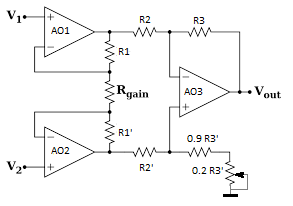
\includegraphics[scale=1.2]{Imagenes/Modificación de R3.png}
  \caption{\textit{Modificación de  R’3.}}
\end{figure}

\hspace{1mm} Dado que las resistencias no se pueden fabricar con una precisión excesiva, para poder conseguir que el último término no degrade la RRMC, se suele hacer que la resistencia \(R'_3 \) varíe su valor de forma que minimice la ganancia en modo común y con ello, maximizar la RRMC.


\section{Costos de los componentes}
\hspace{1mm} A continuación se detallan los costos de los componentes luego de analizar detalladamente el mercado. 

\begin{itemize}
    \item \textbf{Celda de carga CD Flexar SRL:} \(\$ \)66 USD (odoo sipel)
    \item \textbf{Amplificadores LMC6064:} \(\$ \) 5.57 USD (AliExpress)
    \item \textbf{Regulador de tensión REF102:} \(\$ \)0.916 USD (AliExpress)
    \item \textbf{Sensor de temperatura LM35:} \(\$ \)1.79 USD (Mercado Libre)
    \item \textbf{Resistencias de 0.1\(\% \) de tolerancia:} \(\$ \)0.016 USD (Mercado Libre)
    \item \textbf{PIC 18F26J53 con conversor A/D de hasta 12 bits:} \(\$ \)5.23 USD (Digital Key)
    \item \textbf{Presets de 0.1\(\% \) de tolerancia:} \(\$ \)0.27 USD (Digi-key)
\end{itemize}

\hspace{1mm} El precio de cada componente se calculó según el valor unitario. Si se consigue un proveedor fijo para fabricar en masa, el costo se reducirá significativamente.

\section{Conclusión}

\hspace{1mm}Debido al error total de offset (error estático), se debe utilizar un ADC de 12 bits para que cuando se encienda la balanza, por software se pueda llevar este error a cero. Si se mide un valor superior al error máximo de offset, significa que hay alguna masa puesta sobre la balanza (o que algo está averiado en el peor de los casos). 

Con estas consideraciones disminuyen mucho los costos de los componentes ya que se utiliza el software para corregir los errores.

\end{document}